% !TEX root = main.tex
\documentclass{ZJUTbachelor}

%封面、中文摘要信息
\myname{付子航}
\studentid{202203151007}
\major{软件工程}
\thesis{基于混合检索的图表类型推荐系统设计与实现}
\department{计算机科学与技术学院}
\departmentsecond{（软件学院、人工智能学院）}
\mysupervisor{孙国道}
\class{2022软件工程}
\submitdate{2026年6月}

%英文摘要信息
\Enthesis{DESIGN AND IMPLEMENTATION OF A CHART TYPE RECOMMENDATION SYSTEM BASED ON HYBRID RETRIEVAL}



\begin{document}

%——————————————————————————————————————封面—————————————————————————————————————————————————	
	\Cover
%———————————————————————————————————————end—————————————————————————————————————————————————


%——————————————————————————————————————诚信承诺书和任务书—————————————————————————————————————	
	% 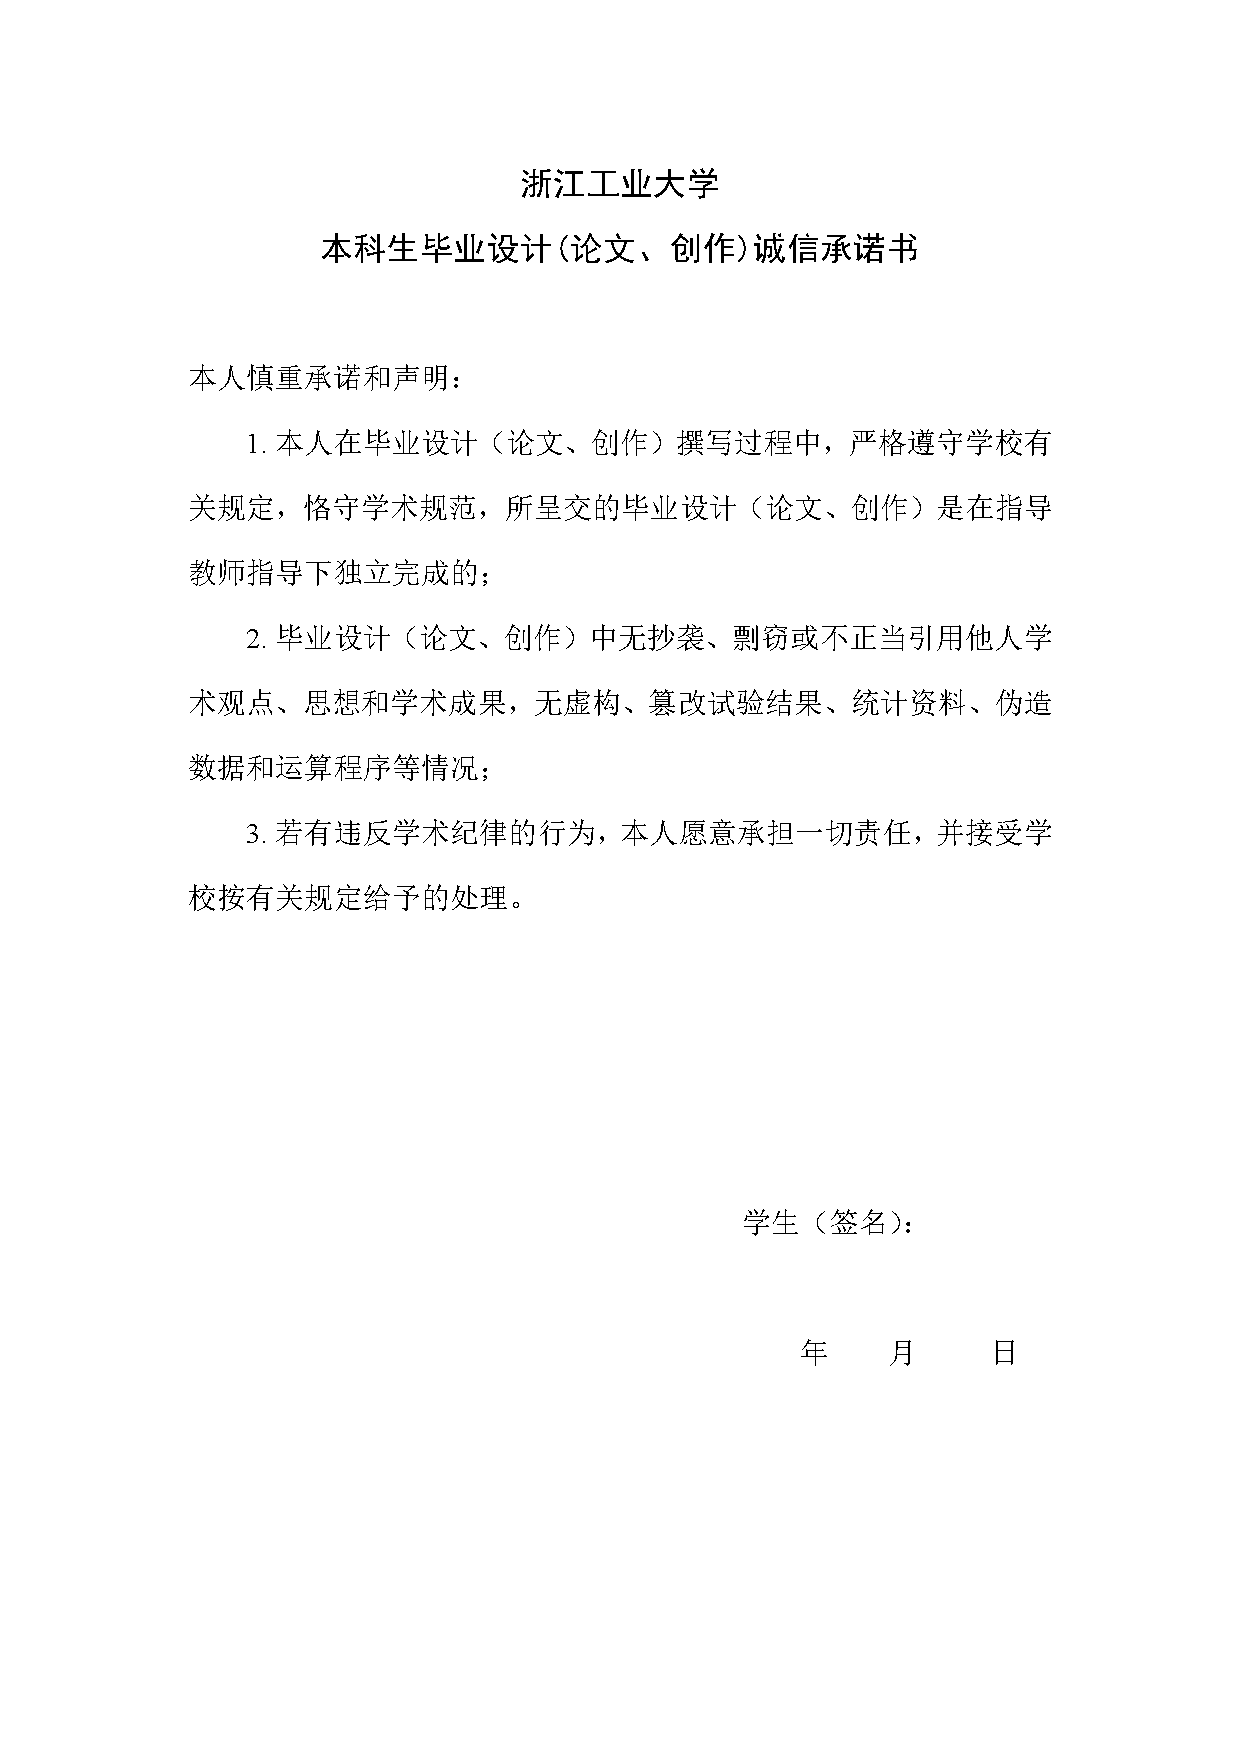
\includepdf{pdf/诚信承诺书.pdf}
	% 
\includepdf{pdf/任务书.pdf}
%———————————————————————————————————————end—————————————————————————————————————————————————


	%页脚罗马数字
	\pagenumbering{Roman}
	
%—————————————————————————————————————中文摘要———————————————————————————————————————————————	
	\ZhAbstract{
		数据可视化已广泛应用于科研分析、商业决策、新闻传播和日常报告写作等场景。对于非专业用户而言，图表制作的困难往往不只来自绘图工具操作，还来自对图表类型适用场景的判断。现有研究较多关注图表绘制、图表理解和可视化美学优化，面向自然语言输入的图表类型推荐仍存在推荐准确性不足、候选结果解释性有限、用户需要反复试错等问题。围绕这一问题，本文研究基于混合检索的图表类型推荐方法，并设计实现一个支持自然语言输入、图表推荐和交互式编辑的原型系统。主要工作包括：
		
		（1）构建面向图表类型推荐任务的 ChartRWC 多模态数据集。针对原始图表数据在类别分布、文本描述完整性和样本可用性方面存在的不足，本文对已有图表数据进行筛选、扩展与规范化整理。该数据集为自然语言查询与图表样例之间的匹配提供了统一的数据基础，也为后续实验提供了可复用的评测对象。
		
		（2）设计基于混合检索的图表类型推荐方法。本文将图表类型推荐建模为自然语言输入与候选图表样例之间的检索排序问题，同时采用稀疏检索和稠密检索两条路径。稀疏检索利用倒排索引和 TF-IDF 表征捕捉文本中的显式关键词线索，适合处理图表名称、数据字段和统计关系等直接匹配信息；稠密检索利用语义向量表示计算查询文本与图表描述之间的语义相似性，补充关键词不完全一致时的匹配能力。在此基础上，本文采用倒数排序融合（Reciprocal Rank Fusion, RRF）算法对两路检索结果进行融合，以提高候选结果的鲁棒性。
		
		（3）实现交互式图表类型推荐原型系统。系统围绕用户从自然语言描述到可视化结果的完整使用流程进行设计，支持用户输入包含数值关系的文本内容，并列查看稀疏检索、稠密检索和 RRF 融合排序产生的候选结果。用户可以根据推荐结果选择合适的图表类型和图表样例，并在图表编辑器中进一步修改数据、标题、颜色等内容。该设计将自动推荐与人工调整结合起来，减少用户在图表类型选择阶段的试错成本，同时保留对最终可视化结果的控制能力。
		
		实验评估结果表明，ChartRWC 中更丰富的图表描述能够提升稀疏检索和稠密检索在图表类型推荐任务中的表现，混合检索结合 RRF 融合排序后能够获得更稳定的候选结果。用户研究结果显示，融合推荐结果在相关性、平均贡献度和准确率等指标上表现较好，参与者也认为并列展示多路推荐结果和提供交互式编辑功能有助于降低图表选择与修改成本。研究结果说明，本文提出的基于混合检索的图表类型推荐流程能够为自然语言驱动的图表生成提供可行路径，并为非专家用户的数据可视化创作提供辅助支持。
	}{图表类型推荐，混合检索，自动图表生成，多模态数据集，数据可视化}
%———————————————————————————————————————end——————————————————————————————————————————————————




%—————————————————————————————————————英文摘要———————————————————————————————————————————————	
	\EnAbstract{Data visualization has been widely used in scientific analysis, business decision-making, public communication, and daily report writing. For non-expert users, the difficulty of creating a chart often lies not only in operating visualization tools, but also in judging which chart type is suitable for the intended use case. Existing studies have mainly focused on chart rendering, chart understanding, and visual design optimization. Chart type recommendation from natural language still faces limitations in recommendation accuracy, result explainability, and repeated trial-and-error by users. To address this problem, this thesis studies a hybrid-retrieval-based chart type recommendation method and implements a prototype system that supports natural language input, chart recommendation, and interactive editing. The main work includes:
	
	(1) A ChartRWC multimodal dataset is constructed for chart type recommendation. To address the limitations of the original chart data in category distribution, description completeness, and sample usability, this thesis filters, extends, and standardizes existing chart data. The dataset provides a unified data basis for matching natural language queries with chart examples and serves as a reusable evaluation object for subsequent experiments.
	
	(2) A hybrid-retrieval-based chart type recommendation method is designed. This thesis formulates chart type recommendation as a retrieval and ranking problem between a natural language input and candidate chart examples, and uses sparse retrieval and dense retrieval in parallel. Sparse retrieval uses an inverted index and TF-IDF representations to capture explicit lexical cues, which is suitable for matching chart names, data fields, and statistical relations. Dense retrieval uses semantic vector representations to measure the similarity between query texts and chart descriptions, complementing sparse retrieval when the wording is not exactly matched. Based on the two retrieval paths, Reciprocal Rank Fusion (RRF) is applied to fuse the retrieval results and improve the robustness of candidate recommendations.
	
	(3) An interactive prototype system is implemented. The system is designed around the complete workflow from natural language description to visual output. It allows users to enter text containing numerical relationships and compare candidate results from sparse retrieval, dense retrieval, and RRF fusion side by side. Users can select appropriate chart types and chart examples from the recommendation results, and then refine data, titles, colors, and other chart elements in the chart editor. This design combines automatic recommendation with manual adjustment, reducing the trial-and-error cost of chart type selection while preserving user control over the final visualization.
	
	Experimental evaluation results show that richer chart descriptions in ChartRWC improve the performance of both sparse retrieval and dense retrieval in the chart type recommendation task, and that combining hybrid retrieval with RRF produces more stable candidate rankings. The user study further shows that the fused recommendation results perform well in terms of relevance, average contribution, and precision. Participants also indicate that displaying multiple retrieval results side by side and providing an interactive editor help reduce the cost of chart selection and refinement. These results suggest that the proposed hybrid-retrieval-based recommendation pipeline provides a feasible path for natural-language-driven chart generation and can support non-expert users in data visualization creation.}{Chart Type Recommendation, Hybrid Retrieval, Automatic Chart Generation, Multimodal Dataset, Data Visualization}
%—————————————————————————————————————————end————————————————————————————————————————————————





%—————————————————————————————————————目录，表列、图列———————————————————————————————————————
	%目录，表列、图列
	\makeTOCandLOTandLOF
	%页码计数器清零，阿拉伯数字
	\setcounter{page}{0}
	\pagenumbering{arabic}
	\newpage
%———————————————————————————————————————end——————————————————————————————————————————————————


	
	
%——————————————————————————————————————正文—————————————————————————————————————————————————	
	\section{绪论}


\subsection{研究动机与目的}

\subsection{研究背景}


\subsection{研究方法}

\subsection{论文内容概述}

\subsubsection{三级标题}

这是三级标题下的正文内容。下面是四级标题和五级标题的示例。

\paragraph{第一个四级标题}

这是第一个四级标题下的内容。四级标题使用 (1)(2)(3) 这样的编号格式。

\subparagraph{第一个五级标题}

这是第一个五级标题下的内容。五级标题使用带圈数字 ① ② ③ 这样的编号格式。

\subparagraph{第二个五级标题}

这是第二个五级标题下的内容。

\paragraph{第二个四级标题}

这是第二个四级标题下的内容。

\subparagraph{第三个五级标题}

这是第三个五级标题下的内容。

\paragraph{第三个四级标题}

这是第三个四级标题下的内容，用于展示编号格式。

\newpage


	\section{相关理论和技术}


\subsection{自动图表生成}

自动图表生成面向的核心问题是如何把用户表达的分析意图稳定地映射为可视化结构。早期研究通常建立在结构化数据输入之上，系统预设字段语义并在候选图表空间内完成匹配与渲染~\cite{dibia_lida_2023}。这一路径在工程实践中具有较高可控性，因为输入模式、图表约束和输出格式都可被显式定义。围绕该路径形成的代表性工作，一部分聚焦“文本到图表”的生成链路~\cite{zhao_ct2c-qa_2024,rashid_text2chart_2022}，另一部分聚焦“表格到可视化”的推理链路~\cite{jain_doc2chart_2025}。两类方法在实现细节上有所差异，但共同前提都指向输入数据具有较好的规整性与可解析性。

当输入由单一表格扩展到文档、图像或多模态线索时，系统能力边界开始显现。已有研究显示，即便引入更强的跨模态理解机制，许多方法仍在不同程度上依赖既有数据结构~\cite{latif_kori_2022,shuai_deepvis_2025}。这种依赖使方法在“结构明确、目标单一”的任务下表现较好~\cite{luo_deepeye_2018,cui_text--viz_2020}，但在“语义含糊、意图混合”的真实写作场景中容易出现推荐失配。根本原因在于，用户文本中的比较关系、强调重点、时间语境和叙述目标往往交织出现，而这些信息难以通过单一字段映射被完整刻画~\cite{masry_unichart_2023}。

研究重心随之由“静态映射”转向“生成与推理协同”。一方面，图表到代码、文本到图表等任务为自动化可视化提供了更完整的工具~\cite{yang_chartmimic_2025,wu_plot2code_2025}；另一方面，多模态大语言模型的快速发展提升了系统对复杂视觉模式与上下文线索的利用能力~\cite{openai_gpt-4vision_2023,gemini_family_2025,anthropic_introducing_2024}。以 LLaVA 系列与 ChartLlama 为代表的工作~\cite{liu_visual_2023,liu_improved_2024,han_chartllama_2023}，以及 Qwen-VL 技术路线~\cite{bai_qwen_technical_2023}，都在一定程度上缓解了早期方法对人工规则的依赖，使系统能够在更弱结构先验下完成图表理解与生成。

尽管如此，现阶段系统在“结构忠实性”与“语义一致性”上的矛盾仍未完全解决。相关研究指出，模型生成的图表代码可能在语法层面可执行，但在数据绑定、图元对应和视觉编码选择上仍出现偏差~\cite{kondic_chartgen_2025}。同时，自然语言驱动的可视化生成虽显著降低了使用门槛~\cite{wang_towards_2022,lu_automatic_2021,wang_making_2023}，却普遍面临图表类型覆盖有限、复杂约束难表达的问题。交互式增强策略能够改善单轮生成不足~\cite{masson_charagraph_2023,zou_gistvis_2025}，但多数系统仍将注意力集中于显式数值信息，对非数值语义和任务意图的建模深度不够。


\subsection{图表数据集}

数据集是图表理解、图表生成与图表推荐任务共同依赖的基础设施，数据组织方式直接影响模型学习到的知识边界~\cite{hu_novachart_2024}。从构建策略看，现有图表数据集可概括为合成数据集、真实世界数据集与混合数据集三类。合成数据集通过程序化管线批量生产样本，在规模扩展、标注一致性和成本控制方面具有明显优势~\cite{kafle_dvqa_2018}。这类数据通常来自在线资源抽取后的再组织~\cite{tang_vistext_2023,akhtar_reading_2023,li_chartgalaxy_2025}，或由大语言模型辅助生成数据语境与任务指令~\cite{xia_chartx_2025,zhao_chartcoder_2025}。对模型训练而言，合成数据能够迅速建立“图形-文本-代码”三者之间的基础映射关系。

合成路径的局限也较为明显。程序化生成过程容易在样式选择、布局策略和叙述语境上形成模板偏置，导致模型在标准样例上表现稳定、在复杂真实样例上泛化不足。与之相比，真实世界数据集覆盖了更多人工设计痕迹与场景噪声，能够更充分反映图表在传播语境中的实际使用形态~\cite{zhou_table2charts_2021}。相关工作从网站平台收集图表样本~\cite{savva_revision_2011,kantharaj_chart--text_2022,masry_chartqa_2022,huang_evochart_2025}，或从出版物与学术资料中提取图表与配套信息~\cite{wu_plot2code_2025,yang_matplotagent_2024,wang_charxiv_2024,zhang_is_2024}，在类型多样性和视觉复杂度上具有优势。问题在于，真实数据通常伴随标注昂贵、质量控制复杂与字段缺失等现实约束，数据规模难以线性提升。

混合数据集因此成为当前较具可行性的折中方案。其核心思路是将合成数据用于扩展规模和覆盖基础模式，将真实数据用于补足分布多样性和语义复杂性，从而在训练阶段形成更平衡的数据分布~\cite{liu_deplot_2023,meng_chartassistant_2024,liu_matcha_2023}。这一路径有助于降低模型对单一数据生成机制的依赖，也有助于提升跨场景迁移能力。对本研究关注的“文本到图表类型推荐”任务而言，混合数据策略同样具有现实意义，因为用户输入文本经常同时包含结构化线索与非结构化语义，需要训练数据能够覆盖两类信息的耦合关系。

从数据形态看，当前图表数据集已从单一图像样本扩展为多模态样本单元，常见组成包括位图、矢量描述、表格数据、文本说明与程序代码。数据字段的丰富化使模型能够在训练中同时学习视觉结构、语言语义与程序表达的对应关系。近期工作继续扩大图表类型覆盖与元数据维度~\cite{wang_omni-chart-600k_2025,liu_mmc_2024}，并在任务层面支持更复杂的生成与理解目标。以 Text2Chart31 为例，其统一描述、代码、数据表与图表的组织方式~\cite{zadeh_text2chart31_2024}，为研究者开展跨模态对齐、可解释推荐与端到端生成提供了更完整的数据基础。


\subsection{图表创作工具}

图表创作工具的发展路线反映了可视化系统从“高效率生产”向“高表达能力与低门槛协同”演进的过程。早期主流工具强调通过界面化配置快速完成标准图表制作，例如 Tableau 等系统通过字段拖拽与视觉通道映射降低了入门难度~\cite{tableau_business_2025}。这类工具在报表场景和常规分析任务中具有较高实用性，但其交互逻辑通常围绕预设图表语法展开，当用户需要表达复杂叙事结构或非常规视觉风格时，扩展能力会受到限制。

后续研究开始将“表达性”作为工具设计的关键目标。Data-Driven Guides、DataInk 和 Data Illustrator 等系统~\cite{kim_data-driven_2016,xia_dataink_2018,liu_data_2018}，通过更细粒度的图形控制机制，使用户能够在数据约束下定义图元关系、重复策略与布局规则。与传统模板式工具相比，这类系统提升了可视化设计空间的可探索性，也使用户能够在准确编码数据的同时兼顾视觉叙事。然而，表达能力提升常常伴随交互复杂度上升，非专家用户在参数理解、约束设置与设计决策上仍需较高学习成本。

编程式可视化工具提供了另一条路径。D3、ECharts 与 Vega-Lite~\cite{bostock_d3_2011,li_echarts_2018,satyanarayan_vega-lite_2016} 通过声明式或命令式方式描述视觉编码逻辑，具备更强可复用性与可扩展性，能够支持交互行为、动画过渡与复杂组合图的精细控制。该路径对工程场景十分友好，适合与 Web 系统、分析平台和自动化流程集成。代价在于，用户需要具备编程基础，并理解图表语法、数据绑定机制与运行环境配置，使用门槛显著高于可视化界面工具。

为了弥合“高表达能力”与“低使用门槛”之间的矛盾，研究者进一步引入草图驱动与检索增强机制。SketchInsight、DataQuilt 等工作~\cite{lee_sketchinsight_2015,zhang_dataquilt_2020} 将原型草图、视觉元素提取与延迟绑定结合起来，支持用户在较弱形式化输入下快速探索设计方向，并在后续阶段补全数据约束。相关研究还通过风格迁移和布局学习提升设计效率~\cite{ma_ladv_2020}，使创作流程由“从零构造”转向“示例引导与局部编辑”。近期方法将视觉编辑与数据驱动生成进一步整合~\cite{coelho_infomages_2020,qian_retrieve-then-adapt_2020}，并使用检索式策略复用已有设计知识，帮助非专家更快获得可接受结果~\cite{shi_supporting_2022}。


\subsection{本章小结}

本章围绕本文研究所依赖的关键理论与技术基础展开梳理。自动图表生成相关研究表明，现有方法在结构化输入场景下已形成较成熟流程，但在真实文本语境中仍面临语义歧义、结构忠实性不足和类型覆盖受限等问题。图表数据集研究显示，合成、真实与混合数据各有优势与边界，数据构建策略正在由单一规模扩张转向规模、质量与任务适配协同优化。图表创作工具的发展则揭示了可视化系统在表达能力与使用门槛之间长期存在的张力，前置推荐机制与后续交互编辑的协同路径具有明确工程价值。基于上述分析，本文后续章节将进一步给出面向文本到图表类型推荐任务的数据构建方案、混合检索方法设计与系统实现细节，以验证所提技术路线的可行性与有效性。

\newpage

	\section{形成性研究}

本文开展了一项形成性研究，以探索数据分析人员在图表创作过程中的挑战与需求。该研究已获得所在机构伦理审查委员会（Institutional Review Board, IRB）的批准，所有收集数据仅用于科学研究目的。参与者在研究开始前均已充分了解研究内容并签署知情同意，同时研究过程保证其数据严格保密，且仅用于本研究。

\subsection{参与者}

本文共招募了11名参与者，其中女性5名、男性6名，平均年龄为31.5岁。参与者按职业背景可分为三类：3名学生（P1-P3）、3名学者（E1、P4、P5）和5名行业从业者（E2、P6-P9）。参与者平均具有9.6年的数据可视化经验。其中，两名专家自愿参与形成性研究，其余参与者在完成研究后获得15美元报酬。参与者的详细信息如表\ref{tab:formative_participant} 所示。

\begin{table}[htbp]
\centering
\caption{形成性研究参与者信息}
\label{tab:formative_participant}
\small
\setlength{\tabcolsep}{3pt}
\begin{tabular}{lllll}
\toprule
参与者 & 身份 & 性别 & 使用场景 & 年龄 \\
\midrule
E1 & 教授 & 男 & 数据可视化、学术写作、数据分析 & 41 \\
E2 & 数据科学家 & 男 & 数据分析 & 43 \\
P1 & 本科生 & 女 & 课程作业、文档写作 & 21 \\
P2 & 硕士研究生 & 女 & 课程作业、文档写作、数据分析 & 24 \\
P3 & 硕士研究生 & 男 & 课程作业、文档写作、数据分析 & 26 \\
P4 & 博士研究生 & 女 & 学术写作、数据分析 & 28 \\
P5 & 博士研究生 & 男 & 学术写作、数据分析 & 31 \\
P6 & 数据叙事从业者 & 女 & 文档写作、数据分析 & 32 \\
P7 & 数据从业者 & 男 & 数据分析 & 33 \\
P8 & 新闻从业者 & 女 & 新闻写作、数据分析 & 33 \\
P9 & 数据从业者 & 男 & 数据分析 & 35 \\
\bottomrule
\end{tabular}
\end{table}

\subsection{研究程序}

本次形成性研究采用半结构化访谈方法，访谈通过线上与线下相结合的方式进行。线上访谈使用飞书或腾讯会议，线下访谈采用面对面交流。每位参与者均接受独立访谈，访谈目标是深入探讨图表推荐功能的必要性。

访谈内容围绕四个核心方面展开：参与者在图表构建方面的个人经验、典型图表创作流程、创作过程中遇到的挑战，以及其评估图表有效性的方法。每次访谈时长为35至60分钟。线上访谈通过视频录制和文字纪要进行记录，线下访谈则通过书面笔记与现场录音结合的方式进行记录。

\subsection{研究发现}

通过收集与分析半结构化访谈数据，本文对参与者反馈进行了系统整理与主题归纳，并提炼出若干关键发现。

\subsubsection{F1：图表选择过载}

访谈结果显示，参与者在选择最合适的数据可视化图表时，经常会产生犹豫或困惑。这种不确定性主要来自可选图表类型过多，使其难以判断哪一种图表最适合当前任务（P1、P4、P6、P8）。虽然参与者熟悉柱状图、折线图和饼图等基础图表，但面对大量选项时，他们往往默认选择这些熟悉类型（P8）。当数据复杂度提高时，用户的不确定性进一步增加，不清楚哪种图表能够更好地呈现数据关系。即使他们知道箱线图、漏斗图等较高级的图表类型，也常因不确定其适用性而避免使用这些图表（P6、P7）。因此，用户往往通过多个基础图表来简化复杂数据，这会导致信息被拆散，难以揭示数据中的深层关系和洞察（P7）。

P6是一位数据叙事从业者，她提到：“我手里有不同渠道的用户来源、转化率和最终消费额数据，我想在一张图里展示这个完整流程以及每个环节的占比，但我完全不知道应该用什么图。最后只能做三个独立的柱状图，但看起来并不容易理解。”

记忆并理解多种图表类型的适用场景本身就是一项专业技能，这对非专家用户或初学者而言会带来较高的认知负担。用户也常担心使用不常见图表会增加与受众沟通的成本，甚至影响他人对其专业性的判断，因此倾向于采取更保守的选择。传统工具（如 Excel）通常将所有图表类型不加区分地展示给用户，缺少足够的引导与上下文信息，反而进一步增加了图表选择难度。

\subsubsection{F2：低效的试错循环}

非专家用户的图表构建过程并不是线性的、由意图驱动的设计流程，而往往表现为低效的试错循环。该过程的典型特征是，用户在数据操作的句法层面与可视化表达的语义层面之间反复切换，其核心机制造成了明显的效率损耗。

这一循环通常从用户基于自身对数据的语义理解和初步分析意图尝试生成图表开始。然而，由于用户心智模型与工具对数据结构的句法要求之间普遍存在差异，初次尝试经常导致视觉编码失败。随后，面对这一障碍，用户的认知焦点会发生显著转移：从“我希望数据表达什么”这一较高层次的语义目标，转向“我应该如何重构数据以满足工具规范”这一较低层次的程序性任务。

P7是一位日常工作中频繁处理数据、但并非可视化设计专家的从业者，他描述道：“我经常为了做一个图，把同一个数据表复制粘贴好几份，用不同格式来尝试，看哪个能生成我想要的图。感觉一半时间都花在这种繁琐工作上。最令人头疼的是，好不容易把图做出来了，老板说‘换个角度展示看看’，然后我又要重复刚才所有步骤。”

这种循环往复的过程不仅大量消耗用户时间，也带来了较重的认知负担，并可能使用户在持续挫败中降低甚至放弃最初的分析目标。因此，最终生成的可视化图表往往并不是数据洞察的最佳视觉表达，而是用户在探索空间中由于时间或认知资源耗尽而选择的“局部最优解”或“满意解”。这一现象揭示出现有可视化工具在引导用户完成从数据到视觉的顺畅映射方面仍存在不足。

\subsubsection{F3：从数据到视觉的转译挑战}

用户在数据可视化过程中面临的核心智力挑战，是完成从特定领域问题到抽象视觉编码的认知跨越。许多情况下，用户清楚自己想通过数据讲述什么故事，或者想回答什么业务问题，例如“如何展示各产品线在不同季度对总销售额的贡献占比”。但是，用户并不清楚如何将这个“故事”或“问题”转译为合适的数据可视化方案，例如“堆叠柱状图”。用户的思维停留在具体业务语境中，而可视化工具的语言是抽象图表类型，二者之间存在难以跨越的鸿沟。

P9是一位数据从业者，他提到：“我知道我想表达什么，我们 A 产品的销售额远超预期，B 产品则没有达标。但我不知道怎么在一张图里把‘实际’、‘目标’和‘差距’这三个信息都清楚展示出来。”

其根本原因在于，非专家用户普遍缺乏一种被称为“可视化素养”（Visualization Literacy）的多层次综合能力。这种素养的核心，是能够将具体业务问题抽象为通用分析任务，例如比较、构成和关系等，并掌握将这些任务映射到最佳视觉编码方案的图式知识。当前主流工具以“图表为中心”的设计范式加剧了这一困境：工具预设用户已经具备这种素养，仅提供执行层面的“图表选项板”，从而在最关键的认知转译环节忽略了非专家用户的核心需求。

\subsubsection{F4：简单化的评价标准}

非专家用户对可视化图表的评价并不主要基于分析层面的严谨性，而是更容易受到审美吸引力和信息传递效率这两个表层修辞目标驱动。前者关注图表是否美观、是否能在汇报或展示中呈现“专业感”；后者则关注观众是否能够快速理解并接受一个预设结论，也就是所谓的“一眼看懂”。因此，图形保真度（如坐标轴完整性）、信息密度以及是否可能引发误读等更深层次的分析质量，往往被忽略。

P8是一位新闻从业者，她说：“我做的图主要是给公众看的，所以最重要的是把结论清楚标出来，让他们一眼就能看到重点，其他信息越少越好。”

这一现象的根源可归结为用户角色目标与专业知识水平的共同作用。在大多数场景下，用户扮演的是“观点传达者”而非“数据探索者”的角色，其核心目标是以最高效率说服观众接受既定结论。这种“修辞”导向的目标，使用户自然会优先选择简洁、美观的设计；而“图形诚信”（Graphical Integrity）原则的普遍缺失，则使他们难以辨别有效简化与误导性失真之间的关键差异，甚至可能在无意识中将“可视化反模式”视为实现高效沟通的捷径。

\subsection{系统设计需求}

基于上述访谈发现，本文提出三项设计原则。这些原则旨在指导智能图表推荐系统的开发，并为用户从意图构建到生成准确、有效的视觉表达提供认知脚手架。

\noindent\textbf{意图先行原则。}
系统的主要交互模型应从询问用户“你想创建什么图表？”转向询问“你想回答什么问题？”（F1、F3）。用户输入包含数值信息的自然语言文本，系统解析其意图并推荐合适图表~\cite{latif2022kori,masry2023unichart,tian2024chartgpt,wang2022towards}。

$\bullet$ \textbf{R1：自然语言意图识别。}
系统必须具备自然语言处理能力，能够准确解析用户输入文本，并从文本中识别核心意图，例如比较数值、观察趋势、探索关系等。

$\bullet$ \textbf{R2：可解释的推荐。}
系统应将推荐结果完整展示给用户，包括被推荐图表的原始案例以及对应排名。

\noindent\textbf{无摩擦探索原则。}
系统设计应尽量降低用户在探索过程中的认知成本和操作成本，从而鼓励迭代优化，而不是让用户在挫败感中妥协（F2）~\cite{luo2021natural}。

$\bullet$ \textbf{R3：并行草稿预览。}
系统应改变串行试错流程，转而同时渲染多个候选视觉编码方案，并以低保真预览形式呈现，使用户能够快速进行横向比较与选择。

$\bullet$ \textbf{R4：探索历史版本比较。}
系统应自动记录探索路径，并以缩略图列表等可视化方式呈现。用户可以随时保存某个满意版本，在不同版本之间进行并排比较，或一键回溯到先前任一状态，从而将线性的“试错-撤销”过程转化为非线性的、可比较的探索过程。

\noindent\textbf{规范化初始状态。}
考虑到系统能力边界，系统输出优化的核心应聚焦于为用户提供一个高质量起点~\cite{stokes2022striking}。这能够在后续用户自定义过程中提供认知支持，而不是执行完全自动化的审查与美化（F4）。

$\bullet$ \textbf{R5：以最佳实践作为默认输出。}
系统基于推荐生成的初始图表必须严格遵循图形诚信与美学设计的最佳实践。例如，柱状图的 Y 轴默认从0开始，默认配色方案应对色盲用户友好，标签应清晰且无重叠。这确保用户图表创作的起点是高质量、无误导的标准模板。

\newpage

	\section{ChartRWC 数据集构建}

本章介绍 ChartRWC 数据集的需求、构建方法以及数据集统计信息。

\subsection{数据集需求}

现有数据驱动式图表推荐方法的成功，在很大程度上依赖于数据集质量~\cite{dibia2019data2vis,hu2019vizml}。本文对学术界常用图表数据集进行了深入调研，例如 ChartQA~\cite{masry2022chartqa}、ChartBench~\cite{Xu2023ChartBench} 和 ChartGen~\cite{kondic2025chartgen}，并识别出以下三个局限：

\begin{itemize}
    \item \textbf{缺乏明确的用户意图：} 这些数据集主要由“数据-图表”对构成，但几乎完全缺少关于选择特定图表背后分析意图的标注。因此，模型难以学习数据与用户深层分析目标之间的映射关系。
    \item \textbf{图表类型分布严重不均：} 在真实世界的数据可视化中，柱状图、折线图和散点图占据了绝大多数实例。因此，现有数据集往往呈现极端类别不平衡，使模型或检索方法在推荐箱线图、雷达图、漏斗图等较少使用的图表类型时表现不佳。
    \item \textbf{数据来源相对同质：} 许多数据集中的表格主要来源于商业报表或科学出版物等特定领域，这限制了模型在处理更广泛领域数据时的泛化能力，例如社交媒体、个人健康等场景。
\end{itemize}

为克服上述不足，本文为 ChartRWC 数据集设定如下三个数据集需求：

\ding{172} \textbf{DR1：足够体量。} 数据集应包含足够的样本规模，以满足检索方法与场景覆盖对数据量的需求。

\ding{173} \textbf{DR2：多样性与平衡性。} 数据集需覆盖真实世界中常见图表类型，并使不同图表类型之间的样本体量保持相对平衡。

\ding{174} \textbf{DR3：广泛的领域覆盖。} 数据集应具有广泛的领域覆盖范围，以增强其泛化能力。

\subsection{数据集构建方法}

为达成第4.1节设定的设计目标，本文采用包含“种子数据收集”与“增强与平衡”的两阶段方法来构建 ChartRWC 数据集。

\subsubsection{种子数据收集}

种子数据主要来源于现有高质量学术数据集，以确保初始数据的准确性和规范性。本文使用公开发布的数据集 ChartGen~\cite{kondic2025chartgen}。该完整数据集包含18种图表类型，并包含结构化数据、图表图像、图表摘要、DocTags、问答对以及代码。

为构建一个能够反映真实世界数据可视化实践并作为稳健基准的数据集，本文首先需要定义本研究的核心图表类型范围。本文没有直接采用 ChartGen 中的全部图表类型，因为其内部样本分布存在显著采集偏差，并且包含许多定义重叠或过于专业化的变体。本文从该数据集中筛选了10种图表类型，并提取源数据、图表图像、问答对和图表描述等核心元素。通过这一流程，最终构建了一个由154,411个样本组成的种子数据集。尽管通过筛选高质量源数据集的方式为种子数据奠定了良好基础，但它仍存在第4.1节所提到的两个关键缺陷。

\textbf{图表类别平衡性不足。}
如表\ref{tab:Statistic} 第二列和第三列所示，最常见的四种图表类型，即折线图、柱状图、箱线图和散点图，占全部种子数据的74.3\%，形成了显著的长尾分布。若以此作为基准，检索方法的整体性能指标可能会被这些高频类别主导。这不仅无法准确评估稀有图表类型上的检索能力，也会削弱其作为公平、全面评测基准的有效性。

\textbf{文本描述语义贫乏。}
绝大多数描述遵循固定模板，其功能仅限于简单识别图表组成元素，而未能传达图表所揭示的核心洞见或叙事。这种语义贫乏会对两种主流检索范式构成明显障碍。对于稀疏检索而言，描述性词汇不足会导致召回率较低；对于稠密检索而言，生成的嵌入向量缺乏区分度，无法与包含真实用户意图的查询在语义空间中有效匹配。

\begin{table}[htbp]
\centering
\small
\resizebox{\textwidth}{!}{
\begin{tabular}{lcccc}
\hline
图表类型 & ChartGen数量 & ChartGen占比(\%) & ChartRWC数量 & ChartRWC占比(\%) \\ \hline
Bar Chart & 28,934 & 18.74 & 17,494 & 9.97 $\downarrow$ \\
Box Plot & 24,664 & 15.97 & 17,498 & 9.98 $\downarrow$ \\
Bubble Plot & 12,188 & 7.89 & 17,482 & 9.97 $\uparrow$ \\
Funnel Chart & 3,657 & 2.37 & 17,293 & 9.86 $\uparrow$ \\
Line Chart & 42,218 & 27.34 & 17,495 & 9.97 $\downarrow$ \\
Pie Chart & 12,969 & 8.40 & 17,486 & 9.97 $\uparrow$ \\
Radar Chart & 5,185 & 3.36 & 17,468 & 9.96 $\uparrow$ \\
Scatter Plot & 18,837 & 12.20 & 17,497 & 9.97 $\downarrow$ \\
Stacked Bar Chart & 1,269 & 0.82 & 16,242 & 9.26 $\uparrow$ \\
Treemap Chart & 4,490 & 2.91 & 19,453 & 11.09 $\uparrow$ \\ \hline
\end{tabular}
}
\caption{ChartGen 与 ChartRWC 的统计信息}
\label{tab:Statistic}
\end{table}

\subsubsection{增强与平衡}

由于种子数据集在图表类型样本数量平衡性和图表文本描述语义丰富度方面存在核心缺陷，本文设计并执行了一套策略性数据集扩展与平衡流程，以达成第4.1节中设定的三项设计目标。该流程包含三种策略：

\ding{172} \textbf{增强数据集异构性。}
为进一步丰富数据的内在多样性并满足异构性目标，本文对种子数据表本身进行了变换，包括列子集选择（通过选取原表列子集创建新表）和数据类型转换（例如，将连续数值变量分箱为类别变量），以增加数据表数量。

\ding{173} \textbf{增加文本描述多样性。}
为增加语义多样性，本文构建了一个主题表，并从中随机抽取主题。随后，将这些主题与图表数据结合，利用 GPT-4o 生成自然语言描述~\cite{chatgpt4o2024}。这些新增描述覆盖了多个真实世界数据分析应用场景。

\ding{174} \textbf{平衡图表类型体量。}
为解决种子数据中的不平衡问题，本文通过减少占比较高图表类型的数量，并增加稀有图表类型的样本数量，缓解数据集中的长尾分布问题。本文设定每种图表类型样本数量约为17,000。对于种子数据中过度表示的图表类型，采用无放回随机下采样方法将其削减至目标比例；对于样本数量不足的图表类型，则使用前述策略\ding{172}和策略\ding{173}生成样本。

该合成过程借助 Matplotlib~\cite{Hunter2007Matplotlib} 和 D3~\cite{bostock2011d3} 等可视化库，基于预定义模板和结构化数据渲染有效样本。通过上述流程，数据集平衡性得到了改善。如表\ref{tab:Statistic} 第三列和第五列所示，占比最低的图表类型从0.82\%提升至9.26\%，而占比最高的图表类型从27.34\%降低至9.97\%。

\subsection{数据集统计与验证}

经过上述两阶段构建流程后，最终 ChartRWC 数据集共包含175,408个样本，如表\ref{tab:Statistic} 所示。其中，部分样本来自种子数据，其余样本由增强与平衡策略生成。每个条目均包含数据表、PNG格式图像、文本描述、问答对以及图表类型标签。

在规模方面，ChartRWC 数据集包含超过17万个样本，足以支撑多模态大语言模型训练，同时也能满足稀疏检索和稠密检索方法的需求（DR1）。在多样性与平衡性方面，如表\ref{tab:Statistic} 所示，与种子数据集相比，ChartRWC 的分布得到了显著改善（DR2）。同时，ChartRWC 数据集也保留并扩展了种子数据的异构性（DR3）。

为验证数据质量，本文邀请2位数据可视化领域参与者（E1、P5）以及3位数据应用领域参与者（P6、P7、P9），对随机抽样的500个样本进行人工评估，每位参与者评估100个样本。评估结果显示，专家认为96.2\%的样本是“合理的”或“非常合理的”，证明了增强与平衡策略的有效性

\newpage

	\section{图表类型推荐系统评估}

在完成数据集构建、混合检索方法设计与系统原型实现后，需要进一步检验本文方法是否能够在推荐效果和用户使用体验两个层面支撑自然语言驱动的图表类型推荐任务。单纯观察系统是否能够返回候选图表并不足以说明方法有效，因为推荐系统既需要在算法层面覆盖正确图表类型，也需要在交互层面帮助用户理解、选择和修改推荐结果。因此，本章围绕“推荐是否准确”和“系统是否有用”两个问题展开评估。

本章评估由消融实验和用户研究两部分组成。消融实验主要考察不同数据集、不同文本表示和不同检索策略对推荐结果的影响，用于分析第三章提出的 ChartRWC 数据集以及第四章提出的混合检索流程是否具有实际贡献。用户研究则从真实使用场景出发，观察参与者在系统辅助下完成图表类型选择和图表编辑的过程，并结合问卷结果分析系统界面与推荐结果的可用性。通过两类评估相互补充，本文能够同时从定量指标和用户反馈两个角度说明系统的有效性与局限。

\subsection{消融实验}

本文设计并实施了两个消融实验，用于验证图表描述质量和训练数据来源对检索推荐效果的影响。实验对象包括第四章提出的稀疏检索和稠密检索两类方法。稀疏检索实验关注文本预处理与图表描述语义质量对关键词匹配的影响，稠密检索实验关注多模态编码模型在不同数据集上训练后能否迁移到另一数据分布。两组实验共同回答一个问题：第三章构建的 ChartRWC 是否比原始 ChartGen 更适合作为自然语言图表推荐任务的数据基础。

实验采用交叉数据集设置。本文分别将 ChartGen 和 ChartRWC 作为候选库构建检索索引或训练表示模型，并在同一数据集和另一数据集上进行测试。这里的“训练集”并不只表示监督学习中的参数训练数据，在稀疏检索中也表示用于建立倒排索引和候选图表库的数据集合；“测试集”表示提供查询文本和真实图表类型标签的数据集合。通过这种设置，实验能够同时观察两种情况：模型或索引在同源数据上的表现，以及面对另一种文本风格和图表分布时的泛化能力。

评价指标采用 Top 1 和 Top 5 准确率。对于每一条测试样本，系统根据输入文本返回一个按相关性排序的候选图表列表，并将候选图表的类型与该测试样本的真实图表类型进行比较。若排名第1的候选图表类型与真实类型一致，则该样本计入 Top 1 命中；若排名前5的候选图表中至少有一个与真实类型一致，则该样本计入 Top 5 命中。对某一图表类型而言，Top 1 或 Top 5 数值等于该类型测试样本中命中样本数占总测试样本数的比例。Top 1 反映系统首位推荐是否准确，Top 5 反映系统是否能在有限候选范围内覆盖正确图表类型。消融实验结果如表\ref{tab:gen2rwc} 和表\ref{tab:rwc2gen} 所示。

\subsubsection{图表描述在稀疏检索中的影响}

稀疏检索实验使用第四章中表现最优的策略3进行词语过滤，即同时剔除实体、停用词、助动词、介词、虚词和标点符号。该设置在固定文本预处理方式的前提下，考察 ChartGen 和 ChartRWC 的图表描述本身是否会影响检索能力。实验中，系统将训练集中的图表描述构建为倒排索引，并使用测试集中的文本描述作为查询。每次查询返回排序后的候选图表，随后根据候选图表类型是否与测试样本真实类型一致计算 Top 1 和 Top 5。

表\ref{tab:gen2rwc} 的列结构可以分为两组。第2列至第5列表示以 ChartGen 作为候选库构建索引时的结果，其中第2、3列是在 ChartGen 自身上测试，第4、5列是在 ChartRWC 上测试；第6列至第9列表示以 ChartRWC 作为候选库构建索引时的结果，其中第6、7列是在 ChartRWC 自身上测试，第8、9列是在 ChartGen 上测试。这样的排列可以直接比较两类能力：同源检索反映数据集内部描述是否足以支持检索，跨数据集检索反映描述是否具有泛化性。

可以发现，当使用 ChartGen 作为训练集时，面对文本描述更复杂的 ChartRWC 数据集，推荐准确率非常低。相反，当使用 ChartRWC 作为训练集时，能够较好完成以 ChartGen 作为测试集的检索任务，并且准确率优于使用 ChartGen 自身作为训练集的情况。除此之外，还存在几个有趣发现：对于箱线图、雷达图和堆叠柱状图，无论 ChartGen 作为训练集还是测试集，其检索成功率均为0；对于柱状图、漏斗图、饼图和散点图，ChartGen 作为测试集时，在 ChartRWC 作为训练集的设置下表现优于以自身作为训练集的设置；对于气泡图，则表现更差。从实验结果可以看出，与 ChartGen 中的图表描述相比，ChartRWC 中的图表描述具有更好的泛化能力。

这一结果与第三章的数据集构建目标一致。ChartGen 的描述更接近模板化摘要，词汇覆盖范围有限，经过策略3过滤后，剩余词项难以充分区分不同图表类型。ChartRWC 的描述包含更多主题词、数值关系和分析语境，即使经过较强过滤，仍能保留与图表类型相关的关键词。因此，以 ChartRWC 为候选库建立倒排索引时，系统更容易从查询文本中捕捉到可匹配线索。气泡图表现下降说明稀疏检索仍然依赖词面线索，当某类图表的描述中实体、变量名或视觉编码表达方式变化较大时，仅靠关键词匹配仍可能不足。

\begin{table}[htbp]
\centering
\caption[策略3下的稀疏检索消融结果]{策略3下的稀疏检索消融结果\zjuttabcaptionen{Sparse Retrieval Ablation Results under Strategy 3}}
\label{tab:gen2rwc}
\tiny
\resizebox{\textwidth}{!}{
\begin{tabular}{lcccccccc}
\toprule
& \multicolumn{8}{c}{策略3} \\
\cmidrule(lr){2-9}
图表类型 & \multicolumn{2}{c}{ChartGen训练} & \multicolumn{2}{c}{ChartRWC测试} & \multicolumn{2}{c}{ChartRWC训练} & \multicolumn{2}{c}{ChartGen测试} \\
\cmidrule(lr){2-3}\cmidrule(lr){4-5}\cmidrule(lr){6-7}\cmidrule(lr){8-9}
& Top1 & Top5 & Top1 & Top5 & Top1 & Top5 & Top1 & Top5 \\
\midrule
Bar Chart & 0.00 & 0.01 & 0.00 & 0.00 & 0.83 & 0.86 & 0.15 & 0.18 \\
Box Plot & 0.00 & 0.00 & 0.00 & 0.00 & 0.93 & 0.93 & 0.00 & 0.00 \\
Bubble Plot & 0.63 & 0.80 & 0.00 & 0.00 & 0.85 & 0.90 & 0.52 & 0.60 \\
Funnel Chart & 0.00 & 0.00 & 0.00 & 0.00 & 0.96 & 0.97 & 0.74 & 0.75 \\
Line Chart & 0.00 & 0.00 & 0.00 & 0.00 & 0.42 & 0.52 & 0.07 & 0.11 \\
Pie Chart & 0.19 & 0.30 & 0.00 & 0.00 & 0.77 & 0.83 & 0.33 & 0.40 \\
Radar Chart & 0.00 & 0.00 & 0.00 & 0.00 & 0.84 & 0.87 & 0.00 & 0.00 \\
Scatter Plot & 0.48 & 0.65 & 0.00 & 0.00 & 0.68 & 0.75 & 0.70 & 0.75 \\
Stacked Bar Chart & 0.00 & 0.00 & 0.00 & 0.00 & 0.56 & 0.70 & 0.00 & 0.00 \\
Treemap Chart & 0.00 & 0.00 & 0.00 & 0.00 & 0.65 & 0.73 & 0.04 & 0.05 \\
\bottomrule
\end{tabular}
}
\end{table}

\subsubsection{图表描述在稠密检索中的影响}

稠密检索实验采用结合文本描述与图表图像的混合编码方式训练 BGE-VL-v1.5-zs 模型。与稀疏检索不同，稠密检索将查询文本和候选图表表示到同一语义空间中，并根据向量相似度进行排序，不直接依赖词项是否完全重合。因此，本实验更关注训练数据能否帮助模型学习图表类型、视觉结构和自然语言描述之间的对应关系。若训练数据中的描述只包含浅层模板信息，模型虽然可以记住部分图表类型特征，但在面对更丰富的用户意图表达时可能泛化不足；若训练数据包含更接近真实查询的语义描述，模型应能更好地处理跨数据集测试。

表\ref{tab:rwc2gen} 的读法与表\ref{tab:gen2rwc} 保持一致。第2列至第5列表示以 ChartGen 作为训练集时的表现，其中包括在 ChartGen 和 ChartRWC 两个测试集上的 Top 1 与 Top 5；第6列至第9列表示以 ChartRWC 作为训练集时的表现，其中包括在 ChartRWC 和 ChartGen 两个测试集上的结果。由于稠密检索需要通过训练得到嵌入表示，本实验中的“训练集”表示用于模型微调的数据来源，“测试集”表示用于生成查询并评价推荐结果的数据来源。

可以发现，当 ChartGen 和 ChartRWC 数据集同时作为训练集和测试集时，检索准确率都较高。但当两个数据集交换作为训练集和测试集时，它们的表现有所不同。对于箱线图、漏斗图、饼图、雷达图和散点图，检索准确率都较好。对于堆叠柱状图和树图，当使用 ChartRWC 作为训练集时表现更好；而柱状图在使用 ChartGen 作为训练集时表现更好。对于折线图，当 ChartGen 作为训练集时，无论使用 ChartGen 自身还是 ChartRWC 作为测试集，检索均失败；而当 ChartRWC 作为训练集时，以 ChartRWC 作为测试集的成功率接近0.9，以 ChartGen 作为测试集的成功率也接近0.4。

稠密检索结果说明，多模态表示能够缓解部分词面差异带来的影响，但训练数据的描述质量仍然决定了模型能否学习稳定的语义边界。箱线图、漏斗图、饼图、雷达图和散点图在跨数据集条件下保持较好表现，说明这些图表类型具有相对明确的视觉结构或语义模式。折线图的差异更明显：使用 ChartGen 训练时，模型几乎无法正确识别折线图；使用 ChartRWC 训练后，折线图在 ChartRWC 测试上的 Top 5 达到0.87，在 ChartGen 测试上也有0.44。这表明 ChartRWC 中更丰富的趋势描述有助于模型学习折线图所对应的时间变化或连续变化语义。

从两组消融实验可以得到较一致的结论。稀疏检索对文本词项更敏感，因此 ChartRWC 的描述扩展直接提升了倒排索引的可用性；稠密检索具备更强语义建模能力，但仍依赖训练数据提供足够清晰的图表-文本对应关系。ChartRWC 在类别平衡和描述丰富度上的改进，使其不仅能提高同源测试中的检索表现，也能在跨数据集测试中表现出更好的迁移能力。后续用户研究因此采用基于 ChartRWC 的混合检索系统作为评估对象，以检验该方法在真实交互场景中的可用性。

\begin{table}[htbp]
\centering
\caption[混合编码稠密检索消融结果]{混合编码稠密检索消融结果\zjuttabcaptionen{Dense Retrieval Ablation Results with Hybrid Encoding}}
\label{tab:rwc2gen}
\tiny
\resizebox{\textwidth}{!}{
\begin{tabular}{lcccccccc}
\toprule
& \multicolumn{8}{c}{文本+图像} \\
\cmidrule(lr){2-9}
图表类型 & \multicolumn{2}{c}{ChartGen训练} & \multicolumn{2}{c}{ChartRWC测试} & \multicolumn{2}{c}{ChartRWC训练} & \multicolumn{2}{c}{ChartGen测试} \\
\cmidrule(lr){2-3}\cmidrule(lr){4-5}\cmidrule(lr){6-7}\cmidrule(lr){8-9}
& Top1 & Top5 & Top1 & Top5 & Top1 & Top5 & Top1 & Top5 \\
\midrule
Bar Chart & 0.89 & 1.00 & 0.46 & 0.85 & 0.88 & 0.90 & 0.19 & 0.41 \\
Box Plot & 1.00 & 1.00 & 0.95 & 0.98 & 0.97 & 0.97 & 0.96 & 0.96 \\
Bubble Plot & 1.00 & 1.00 & 0.66 & 0.86 & 0.59 & 0.60 & 0.56 & 0.59 \\
Funnel Chart & 1.00 & 1.00 & 1.00 & 1.00 & 0.98 & 0.98 & 0.96 & 0.96 \\
Line Chart & 0.00 & 0.00 & 0.00 & 0.00 & 0.84 & 0.87 & 0.37 & 0.44 \\
Pie Chart & 1.00 & 1.00 & 0.89 & 0.99 & 0.97 & 0.97 & 0.96 & 1.00 \\
Radar Chart & 1.00 & 1.00 & 0.91 & 0.95 & 0.99 & 0.99 & 1.00 & 1.00 \\
Scatter Plot & 0.96 & 0.96 & 0.83 & 0.95 & 0.74 & 0.75 & 0.81 & 0.89 \\
Stacked Bar Chart & 0.89 & 1.00 & 0.19 & 0.55 & 0.94 & 0.96 & 0.81 & 0.85 \\
Treemap Chart & 0.78 & 0.89 & 0.29 & 0.47 & 0.85 & 0.85 & 0.93 & 0.96 \\
\bottomrule
\end{tabular}
}
\end{table}

\subsection{用户研究}

本文额外招募了15名大学生和研究生参与用户研究（7名男性、8名女性，平均年龄22.5岁），且与第3.1节中的参与者无重叠。该研究已获得所在学校机构审查委员会批准。所有参与者均签署知情同意书，并被告知其数据将被严格保密且仅用于本研究目的。所有参与者均具备数据分析经验，例如曾在课程或项目中使用 Excel 或 Python 进行数据可视化。每位参与者在完成研究后获得10美元报酬。本文分别通过定量方式验证推荐图表类型的准确性，并通过定性方式评估用户对系统的主观感受。实验步骤如下：

\textbf{步骤1：} 向参与者简要介绍本文工作的目标和系统使用方式，确保其了解实验目的与流程。研究人员演示如何使用图表推荐系统，回答参与者问题，并确保参与者熟悉操作。（5-10分钟）

\textbf{步骤2：} 向参与者展示10个包含数值数据的文本描述，这些数据不包含在 ChartRWC 数据库中。推荐系统根据输入文本描述建议最多5种图表类型。参与者选择最能传达文本描述含义的图表类型。研究人员记录推荐图表的显示顺序和参与者选择，并使用期望倒数排名（Expected Reciprocal Rank, ERR）算法~\cite{chapelle2009expected} 评估结果。（20-30分钟）

\textbf{步骤3：} 要求参与者填写反馈问卷，重点评估其使用图表推荐系统的体验。问卷使用1-5分李克特量表评估推荐准确性、推荐多样性、图表相关性、界面易用性和整体满意度，其中1表示“非常不同意”，5表示“非常同意”。此外，参与者可以提供改进建议，以帮助优化系统功能与用户体验。（5-10分钟）

\begin{figure}[htbp]
    \centering
    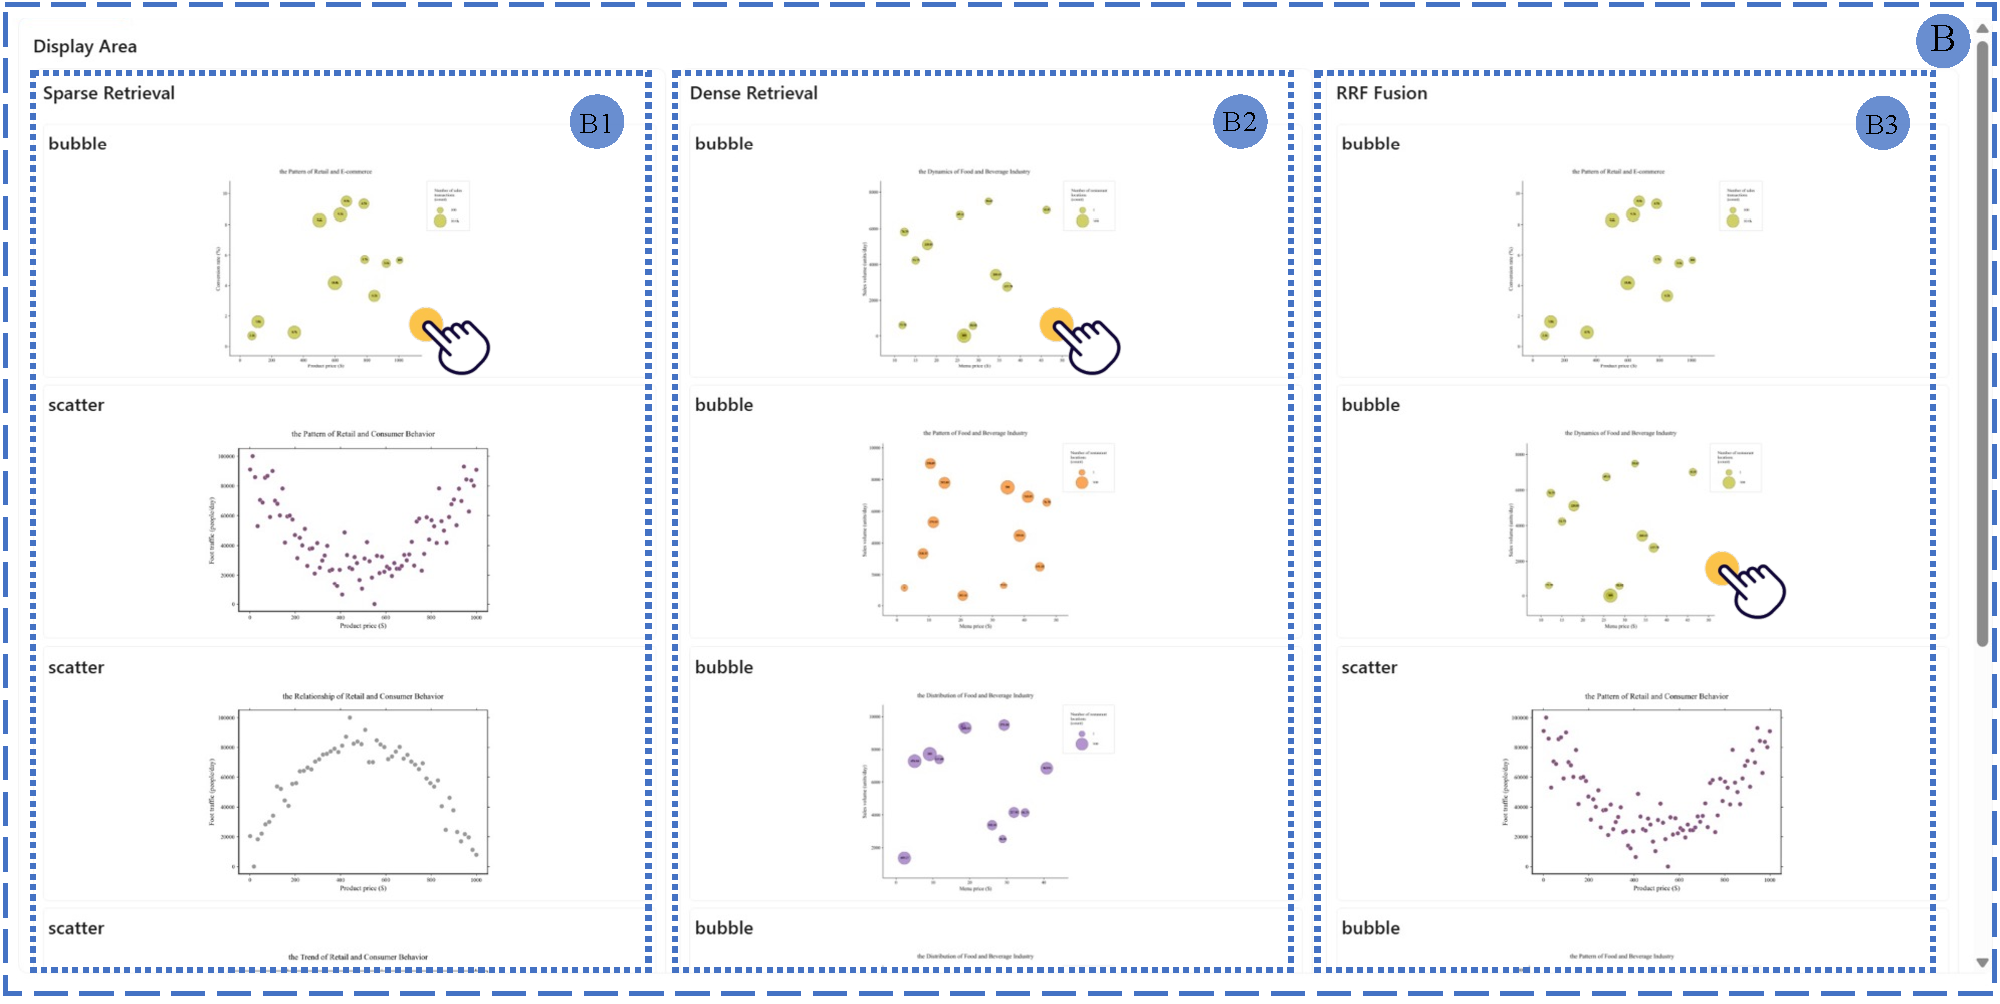
\includegraphics[width=\linewidth]{pics/Display_area.pdf}
    \caption[检索结果展示区]{检索结果展示区\zjutfigcaptionen{Retrieval Result Display Area}}
    \label{fig:display_area}
\end{figure}

\subsubsection{图表推荐准确性}

推荐系统如图\ref{fig:teaser} 所示。用户首先输入想要可视化的文本（A），然后点击“推荐”按钮。检索结果显示在展示区（B），其中（B1）显示稀疏检索结果，（B2）显示稠密检索结果，（B3）显示通过 RRF 算法融合后的推荐结果。

在步骤2中，用户根据自身需求，分别从（B1）、（B2）和（B3）中选择最合适的图表类型。用户选择的图表类型作为系统推荐反馈，用于进一步评估推荐准确性。为了从不同角度衡量三种推荐方法，本文采用平均相关性、平均贡献度（ERR）和准确率三个指标。三者的侧重点不同：平均相关性关注推荐列表整体是否与输入文本相关；ERR 关注合适图表在推荐列表中的排序位置；准确率关注推荐结果是否命中用户最终认可的图表类型。

平均相关性用于衡量推荐列表整体与输入文本语义之间的匹配程度。参与者在比较每种方法给出的 Top 5 推荐结果后，对推荐结果是否适合表达当前文本中的数值关系进行相关性判断，相关性评分被归一化到 $[0,1]$ 区间。设测试文本数量为 $N$，参与者数量为 $P$，推荐方法为 $m$，第 $n$ 个文本由第 $p$ 名参与者给出的相关性评分为 $Rel_{n,p}^{(m)}$，则方法 $m$ 的平均相关性计算为：

\begin{equation}
    AvgRel^{(m)} = \frac{1}{NP}\sum_{n=1}^{N}\sum_{p=1}^{P} Rel_{n,p}^{(m)}
\end{equation}

平均相关性越高，说明该方法返回的候选图表整体越能贴合输入文本的语义和数据关系，但该指标不区分相关图表出现在第1位还是第5位。

平均贡献度使用期望倒数排名（Expected Reciprocal Rank, ERR）计算。ERR 通过衡量用户选择图表与推荐图表之间的匹配情况，并综合考虑推荐序列中的排名信息，为系统提供定量排序评估。ERR 算法的数学表达如下：

\begin{equation}
    ERR = \sum_{i=1}^{K} \frac{1}{i} R_i\prod_{j=1}^{i-1} (1 - R_j)
\end{equation}

其中，$K$ 表示推荐图表数量，本文取 $K=5$。$i$ 表示当前正在评估的图表位置。$R_i$ 表示第 $i$ 个推荐图表是否与用户选择匹配的指示函数；当 $R_i=1$ 时，表示第 $i$ 个推荐图表与用户选择一致；当 $R_i=0$ 时，表示不一致。$\prod_{j=1}^{i-1}(1-R_j)$ 确保在第 $i$ 个推荐图表之前，所有图表均未与用户选择匹配。因此，如果用户认可的图表出现在第1位，则 ERR 取值最高；如果该图表出现在较靠后的位置，则贡献按 $\frac{1}{i}$ 衰减；如果 Top 5 中没有匹配图表，则该轮 ERR 为0。表\ref{tab:err} 中的平均贡献度 $Ave_{ERR}$ 是所有测试文本和参与者对应 ERR 值的平均结果。

准确率用于统计推荐结果是否命中用户最终认可的图表类型。对于每个测试文本，若某种方法给出的 Top 5 推荐列表中包含用户选择的图表类型，则记为命中；否则记为未命中。设命中指示变量为 $Hit_{n,p}^{(m)}$，则方法 $m$ 的准确率为：

\begin{equation}
    Precision^{(m)} = \frac{1}{NP}\sum_{n=1}^{N}\sum_{p=1}^{P} Hit_{n,p}^{(m)}
\end{equation}

准确率反映推荐列表是否覆盖用户需要的图表类型，但不考虑该图表在列表中的具体排名。因此，若两个方法准确率相同，ERR 更高的方法通常代表其排序质量更好。

本文计算稀疏检索、稠密检索和 RRF 融合推荐结果的平均相关性、平均贡献度（ERR）以及准确率，如表\ref{tab:err} 所示。从中可以看出，RRF 在相关性、平均贡献度和准确率上均表现优秀，是最能满足用户需求的推荐方法；稠密检索在平均贡献度和准确率上略低于 RRF；稀疏检索在三个方面仍有提升空间。

\begin{table}[htbp]
\centering
\caption[推荐方法评估结果]{推荐方法评估结果\zjuttabcaptionen{Evaluation Results of Recommendation Methods}}
\label{tab:err}
\begin{tabular}{cccc}
\toprule
推荐方法 & 平均相关性 & 平均贡献度($Ave_{ERR}$) & 准确率 \\
\midrule
稀疏检索 & 0.78 & 0.62 & 80\% \\
稠密检索 & 0.82 & 0.68 & 85\% \\
RRF & 0.84 & 0.72 & 90\% \\
\bottomrule
\end{tabular}
\end{table}

\subsubsection{用户体验评估}

完成实验步骤3后，本文收集了15名参与者的调查问卷，并对收集到的问卷进行统计，结果如图\ref{fig:userstudy} 所示。问卷采用5分制李克特量表，共包含5个问题。关于推荐准确性（Q1），参与者的主观感受与第5.2.1节中的结论一致，约73\%的参与者认为实验过程中 RRF 推荐结果最符合其需求。参与者认为三种推荐方法给出的结果多样性相近（Q2），这可能也与数据集中图表种类数量有限有关。在推荐图表与输入文本相关性方面，几乎所有参与者都认为 RRF 给出的推荐高度相关（Q3）。在系统可用性和整体满意度方面，大部分参与者给出了正面评价（Q4、Q5）。

\begin{figure}[htbp]
    \centering
    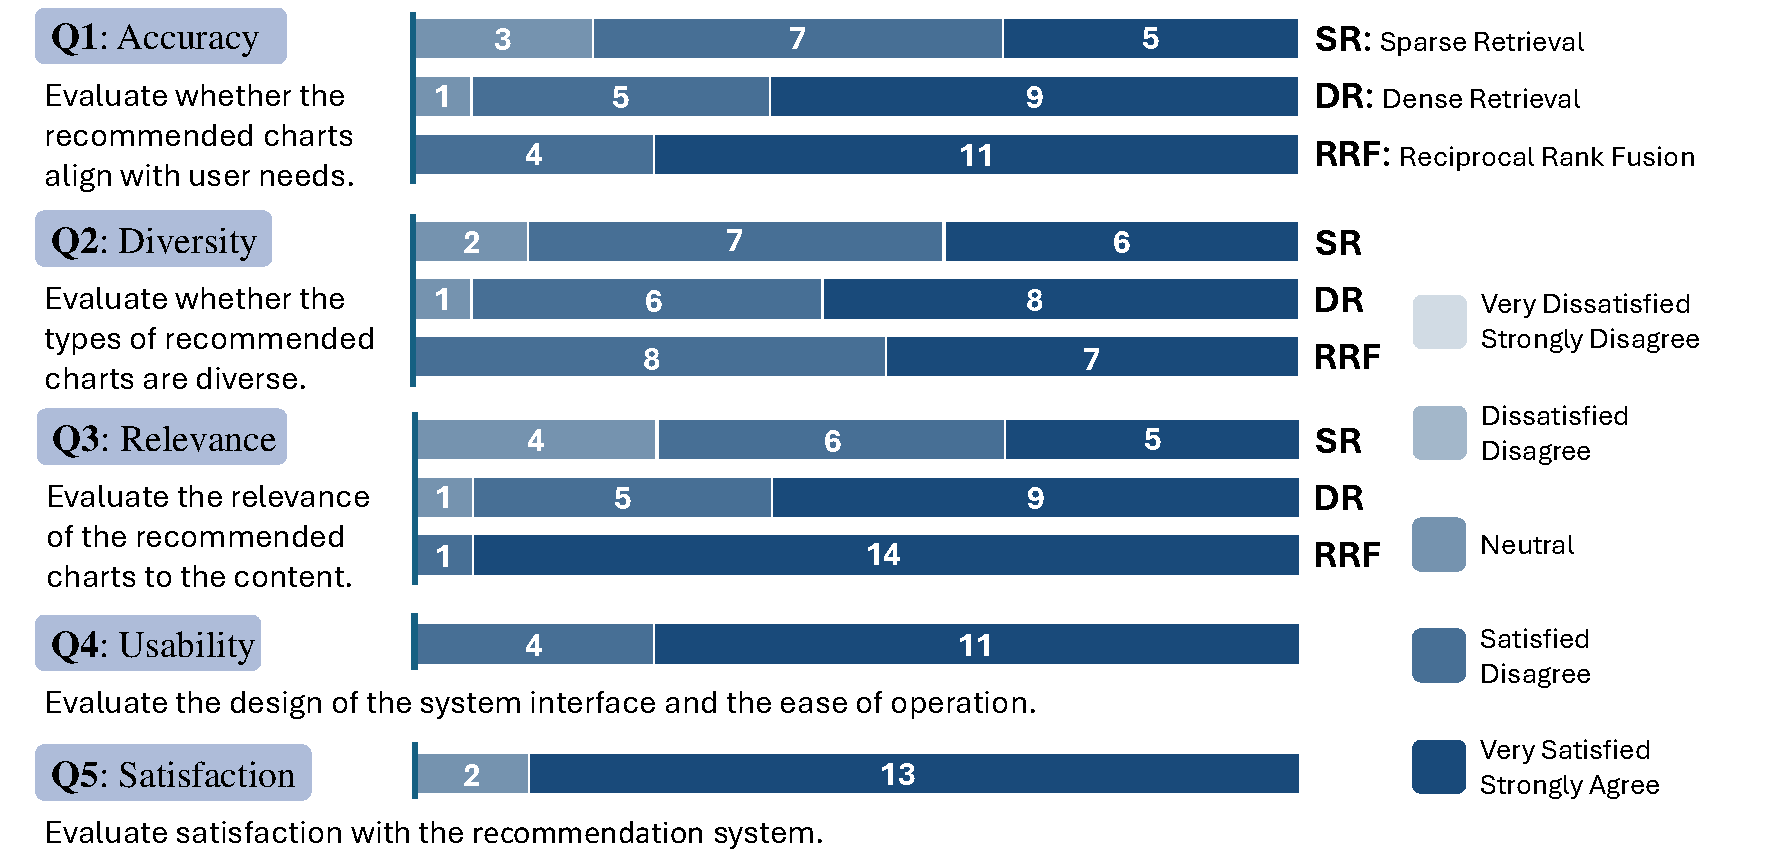
\includegraphics[width=0.8\linewidth]{pics/user_study.png}
    \caption[用户研究问卷结果]{用户研究问卷结果\zjutfigcaptionen{User Study Questionnaire Results}}
    \label{fig:userstudy}
\end{figure}

本文还收集了参与者对推荐系统的开放性反馈，以更好了解其看法和建议。参与者普遍认为该系统使用起来非常方便。用户只需输入文本，系统即可推荐适合体现该文本中数值信息的图表（R1）；三种推荐算法的结果按列排列，也能够帮助数据科学初学者更好理解和解释推荐结果（R2）。参与者喜欢系统编辑区一开始给出初始图表（R5），因为这样不会削弱数据分析的乐趣。他们认为，制图不应完全自动化，因为自动化虽然可以节省体力劳动，但也可能限制创造力。通过算法和系统提供建议，帮助数据分析人员或图表制作者反复迭代和修改（R4），已经能够满足他们的需求和心理预期。

\newpage




	\section{评估}

本章组织消融实验与用户研究，并对结果进行分析。

\subsection{消融实验}

本文设计并实施了两个消融实验，用于验证不同图表描述对（1）稀疏检索和（2）稠密检索的影响。在消融实验中，本文分别使用 ChartGen 和 ChartRWC 作为训练集，然后将另一个数据集作为测试集。消融实验结果如表\ref{tab:gen2rwc} 和表\ref{tab:rwc2gen} 所示。

\subsubsection{图表描述在稀疏检索中的影响}

本文使用策略3进行词语过滤。表\ref{tab:gen2rwc} 第2列至第5列表示以 ChartGen 作为训练集，并分别使用 ChartGen 和 ChartRWC 作为测试集；第6列至第9列表示以 ChartRWC 作为训练集，并分别使用 ChartRWC 和 ChartGen 作为测试集。

可以发现，当使用 ChartGen 作为训练集时，面对文本描述更复杂的 ChartRWC 数据集，推荐准确率非常低。相反，当使用 ChartRWC 作为训练集时，能够较好完成以 ChartGen 作为测试集的检索任务，并且准确率优于使用 ChartGen 自身作为训练集的情况。除此之外，还存在几个有趣发现：对于箱线图、雷达图和堆叠柱状图，无论 ChartGen 作为训练集还是测试集，其检索成功率均为0；对于柱状图、漏斗图、饼图和散点图，ChartGen 作为测试集时，在 ChartRWC 作为训练集的设置下表现优于以自身作为训练集的设置；对于气泡图，则表现更差。从实验结果可以看出，与 ChartGen 中的图表描述相比，ChartRWC 中的图表描述具有更好的泛化能力。

\begin{table}[htbp]
\centering
\caption{策略3下的稀疏检索消融结果}
\label{tab:gen2rwc}
\tiny
\resizebox{\textwidth}{!}{
\begin{tabular}{lcccccccc}
\toprule
& \multicolumn{8}{c}{策略3} \\
\cmidrule(lr){2-9}
图表类型 & \multicolumn{2}{c}{ChartGen训练} & \multicolumn{2}{c}{ChartRWC测试} & \multicolumn{2}{c}{ChartRWC训练} & \multicolumn{2}{c}{ChartGen测试} \\
\cmidrule(lr){2-3}\cmidrule(lr){4-5}\cmidrule(lr){6-7}\cmidrule(lr){8-9}
& Top1 & Top5 & Top1 & Top5 & Top1 & Top5 & Top1 & Top5 \\
\midrule
Bar Chart & 0.00 & 0.01 & 0.00 & 0.00 & 0.83 & 0.86 & 0.15 & 0.18 \\
Box Plot & 0.00 & 0.00 & 0.00 & 0.00 & 0.93 & 0.93 & 0.00 & 0.00 \\
Bubble Plot & 0.63 & 0.80 & 0.00 & 0.00 & 0.85 & 0.90 & 0.52 & 0.60 \\
Funnel Chart & 0.00 & 0.00 & 0.00 & 0.00 & 0.96 & 0.97 & 0.74 & 0.75 \\
Line Chart & 0.00 & 0.00 & 0.00 & 0.00 & 0.42 & 0.52 & 0.07 & 0.11 \\
Pie Chart & 0.19 & 0.30 & 0.00 & 0.00 & 0.77 & 0.83 & 0.33 & 0.40 \\
Radar Chart & 0.00 & 0.00 & 0.00 & 0.00 & 0.84 & 0.87 & 0.00 & 0.00 \\
Scatter Plot & 0.48 & 0.65 & 0.00 & 0.00 & 0.68 & 0.75 & 0.70 & 0.75 \\
Stacked Bar Chart & 0.00 & 0.00 & 0.00 & 0.00 & 0.56 & 0.70 & 0.00 & 0.00 \\
Treemap Chart & 0.00 & 0.00 & 0.00 & 0.00 & 0.65 & 0.73 & 0.04 & 0.05 \\
\bottomrule
\end{tabular}
}
\end{table}

\subsubsection{图表描述在稠密检索中的影响}

本文采用结合文本描述与图表图像的混合编码方式训练 BGE-VL-v1.5-zs 模型。表\ref{tab:rwc2gen} 第2列至第5列表示以 ChartGen 作为训练集，并分别使用 ChartGen 和 ChartRWC 作为测试集；第6列至第9列表示以 ChartRWC 作为训练集，并分别使用 ChartRWC 和 ChartGen 作为测试集。

可以发现，当 ChartGen 和 ChartRWC 数据集同时作为训练集和测试集时，检索准确率都较高。但当两个数据集交换作为训练集和测试集时，它们的表现有所不同。对于箱线图、漏斗图、饼图、雷达图和散点图，检索准确率都较好。对于堆叠柱状图和树图，当使用 ChartRWC 作为训练集时表现更好；而柱状图在使用 ChartGen 作为训练集时表现更好。对于折线图，当 ChartGen 作为训练集时，无论使用 ChartGen 自身还是 ChartRWC 作为测试集，检索均失败；而当 ChartRWC 作为训练集时，以 ChartRWC 作为测试集的成功率接近0.9，以 ChartGen 作为测试集的成功率也接近0.4。

\begin{table}[htbp]
\centering
\caption{混合编码稠密检索消融结果}
\label{tab:rwc2gen}
\tiny
\resizebox{\textwidth}{!}{
\begin{tabular}{lcccccccc}
\toprule
& \multicolumn{8}{c}{文本+图像} \\
\cmidrule(lr){2-9}
图表类型 & \multicolumn{2}{c}{ChartGen训练} & \multicolumn{2}{c}{ChartRWC测试} & \multicolumn{2}{c}{ChartRWC训练} & \multicolumn{2}{c}{ChartGen测试} \\
\cmidrule(lr){2-3}\cmidrule(lr){4-5}\cmidrule(lr){6-7}\cmidrule(lr){8-9}
& Top1 & Top5 & Top1 & Top5 & Top1 & Top5 & Top1 & Top5 \\
\midrule
Bar Chart & 0.89 & 1.00 & 0.46 & 0.85 & 0.88 & 0.90 & 0.19 & 0.41 \\
Box Plot & 1.00 & 1.00 & 0.95 & 0.98 & 0.97 & 0.97 & 0.96 & 0.96 \\
Bubble Plot & 1.00 & 1.00 & 0.66 & 0.86 & 0.59 & 0.60 & 0.56 & 0.59 \\
Funnel Chart & 1.00 & 1.00 & 1.00 & 1.00 & 0.98 & 0.98 & 0.96 & 0.96 \\
Line Chart & 0.00 & 0.00 & 0.00 & 0.00 & 0.84 & 0.87 & 0.37 & 0.44 \\
Pie Chart & 1.00 & 1.00 & 0.89 & 0.99 & 0.97 & 0.97 & 0.96 & 1.00 \\
Radar Chart & 1.00 & 1.00 & 0.91 & 0.95 & 0.99 & 0.99 & 1.00 & 1.00 \\
Scatter Plot & 0.96 & 0.96 & 0.83 & 0.95 & 0.74 & 0.75 & 0.81 & 0.89 \\
Stacked Bar Chart & 0.89 & 1.00 & 0.19 & 0.55 & 0.94 & 0.96 & 0.81 & 0.85 \\
Treemap Chart & 0.78 & 0.89 & 0.29 & 0.47 & 0.85 & 0.85 & 0.93 & 0.96 \\
\bottomrule
\end{tabular}
}
\end{table}

\subsection{用户研究}

本文额外招募了15名大学生和研究生参与用户研究（7名男性、8名女性，平均年龄22.5岁），且与第3.1节中的参与者无重叠。该研究已获得所在学校机构审查委员会批准。所有参与者均签署知情同意书，并被告知其数据将被严格保密且仅用于本研究目的。所有参与者均具备数据分析经验，例如曾在课程或项目中使用 Excel 或 Python 进行数据可视化。每位参与者在完成研究后获得10美元报酬。本文分别通过定量方式验证推荐图表类型的准确性，并通过定性方式评估用户对系统的主观感受。实验步骤如下：

\textbf{步骤1：} 向参与者简要介绍本文工作的目标和系统使用方式，确保其了解实验目的与流程。研究人员演示如何使用图表推荐系统，回答参与者问题，并确保参与者熟悉操作。（5-10分钟）

\textbf{步骤2：} 向参与者展示10个包含数值数据的文本描述，这些数据不包含在 ChartRWC 数据库中。推荐系统根据输入文本描述建议最多5种图表类型。参与者选择最能传达文本描述含义的图表类型。研究人员记录推荐图表的显示顺序和参与者选择，并使用期望倒数排名（Expected Reciprocal Rank, ERR）算法~\cite{chapelle2009expected} 评估结果。（20-30分钟）

\textbf{步骤3：} 要求参与者填写反馈问卷，重点评估其使用图表推荐系统的体验。问卷使用1-5分李克特量表评估推荐准确性、推荐多样性、图表相关性、界面易用性和整体满意度，其中1表示“非常不同意”，5表示“非常同意”。此外，参与者可以提供改进建议，以帮助优化系统功能与用户体验。（5-10分钟）

\begin{figure}[htbp]
    \centering
    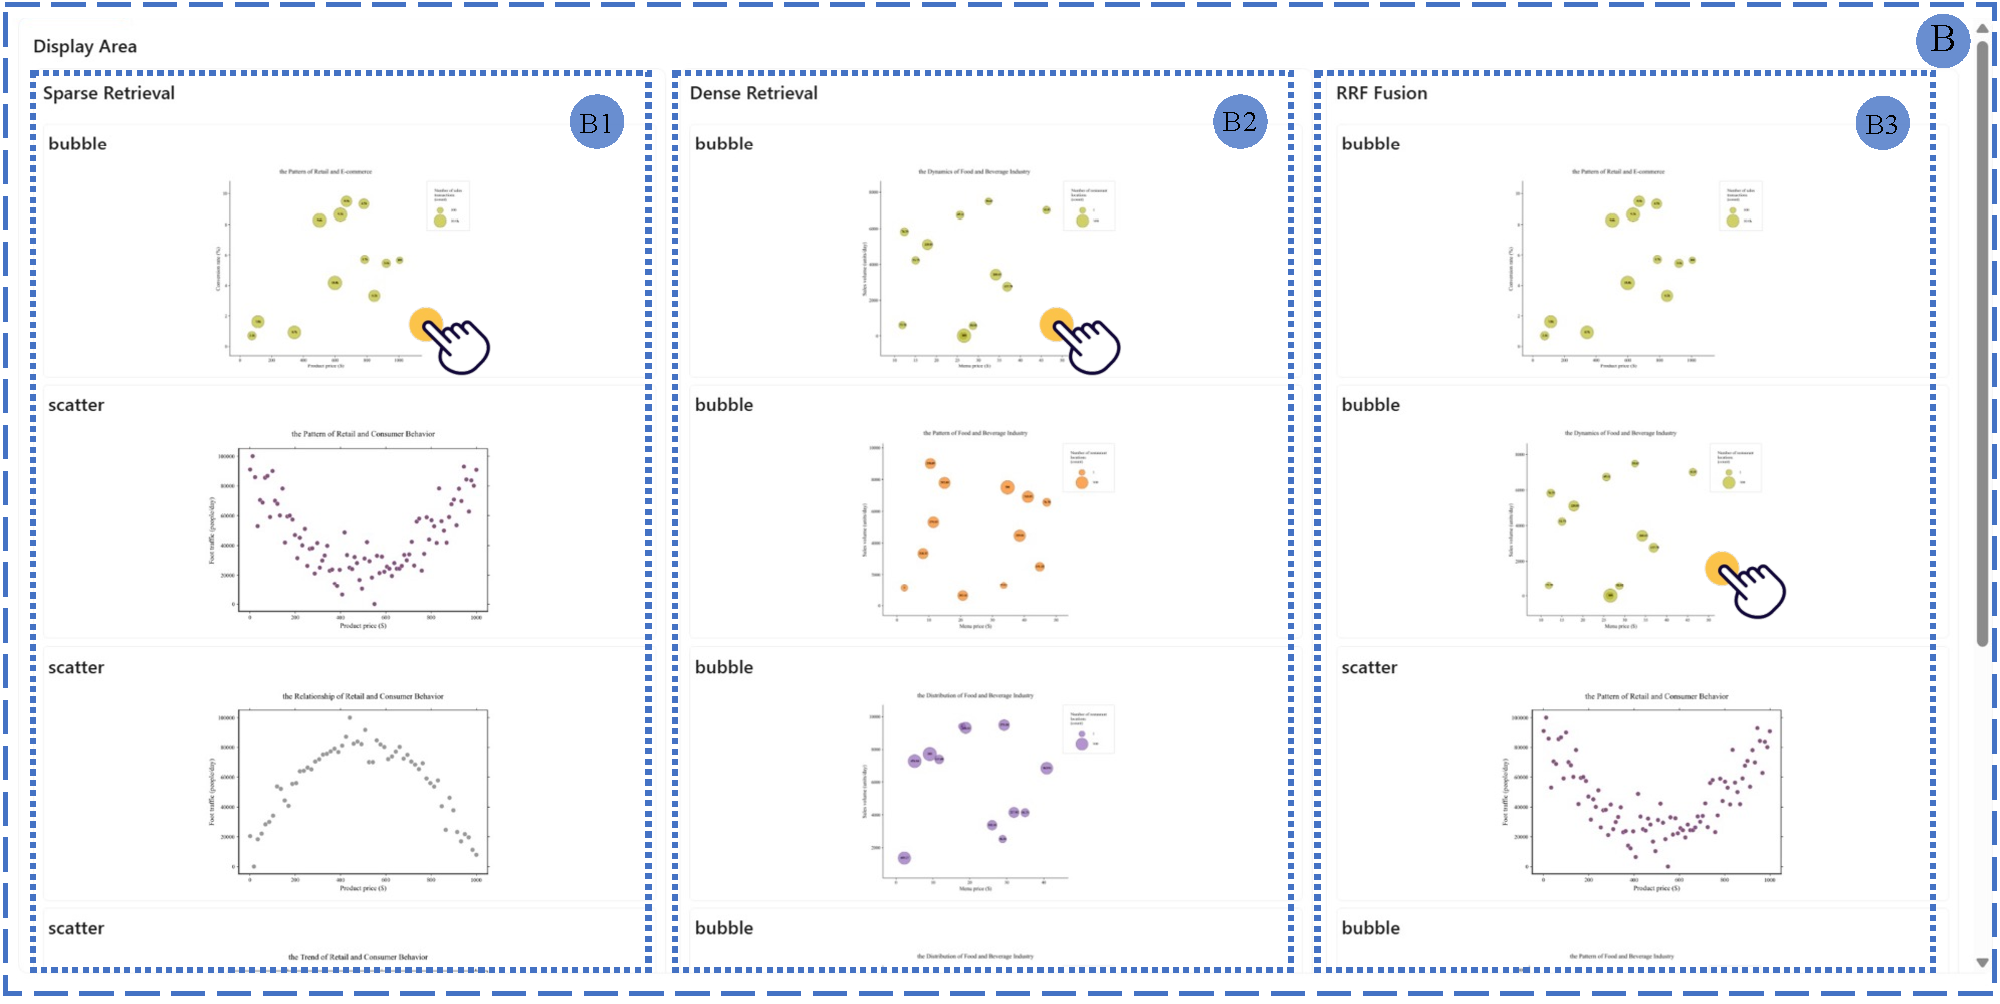
\includegraphics[width=\linewidth]{pics/Display_area.pdf}
    \caption{检索结果展示区}
    \label{fig:placeholder}
\end{figure}

\subsubsection{图表推荐准确性}

推荐系统如图\ref{fig:teaser} 所示。用户首先输入想要可视化的文本（A），然后点击“推荐”按钮。检索结果显示在展示区（B），其中（B1）显示稀疏检索结果，（B2）显示稠密检索结果，（B3）显示通过 RRF 算法融合后的推荐结果。

在步骤2中，用户根据自身需求，分别从（B1）、（B2）和（B3）中选择最合适的图表类型。用户选择的图表类型作为系统推荐反馈，用于进一步评估推荐准确性。在实验中，本文使用 ERR 算法计算推荐准确性。ERR 算法通过衡量用户选择图表与推荐图表之间的匹配情况，并综合考虑推荐序列中的排名信息，为系统提供定量准确性评估。ERR 算法的数学表达如下：

\begin{equation}
    ERR = \sum_{i=1}^{K} \frac{1}{i} R_i\prod_{j=1}^{i-1} (1 - R_j)
\end{equation}

其中，$K$ 表示推荐图表数量，本文取 $K=5$。$i$ 表示当前正在评估的图表位置。$R_i$ 表示第 $i$ 个推荐图表是否与用户选择匹配的指示函数；当 $R_i=1$ 时，表示第 $i$ 个推荐图表与用户选择一致；当 $R_i=0$ 时，表示不一致。$\prod_{j=1}^{i-1}(1-R_j)$ 确保在第 $i$ 个推荐图表之前，所有图表均未与用户选择匹配。

本文计算稀疏检索、稠密检索和 RRF 融合推荐结果的平均相关性、平均贡献度（ERR）以及准确率，如表\ref{tab:err} 所示。从中可以看出，RRF 在相关性、平均贡献度和准确率上均表现优秀，是最能满足用户需求的推荐方法；稠密检索在平均贡献度和准确率上略低于 RRF；稀疏检索在三个方面仍有提升空间。

\begin{table}[htbp]
\centering
\caption{推荐方法评估结果}
\label{tab:err}
\begin{tabular}{cccc}
\toprule
推荐方法 & 平均相关性 & 平均贡献度($Ave_{ERR}$) & 准确率 \\
\midrule
稀疏检索 & 0.78 & 0.62 & 80\% \\
稠密检索 & 0.82 & 0.68 & 85\% \\
RRF & 0.84 & 0.72 & 90\% \\
\bottomrule
\end{tabular}
\end{table}

\subsubsection{用户体验评估}

完成实验步骤3后，本文收集了15名参与者的调查问卷，并对收集到的问卷进行统计，结果如图\ref{fig:userstudy} 所示。问卷采用5分制李克特量表，共包含5个问题。关于推荐准确性（Q1），参与者的主观感受与第6.2.1节中的结论一致，约73\%的参与者认为实验过程中 RRF 推荐结果最符合其需求。参与者认为三种推荐方法给出的结果多样性相近（Q2），这可能也与数据集中图表种类数量有限有关。在推荐图表与输入文本相关性方面，几乎所有参与者都认为 RRF 给出的推荐高度相关（Q3）。在系统可用性和整体满意度方面，大部分参与者给出了正面评价（Q4、Q5）。

\begin{figure}[htbp]
    \centering
    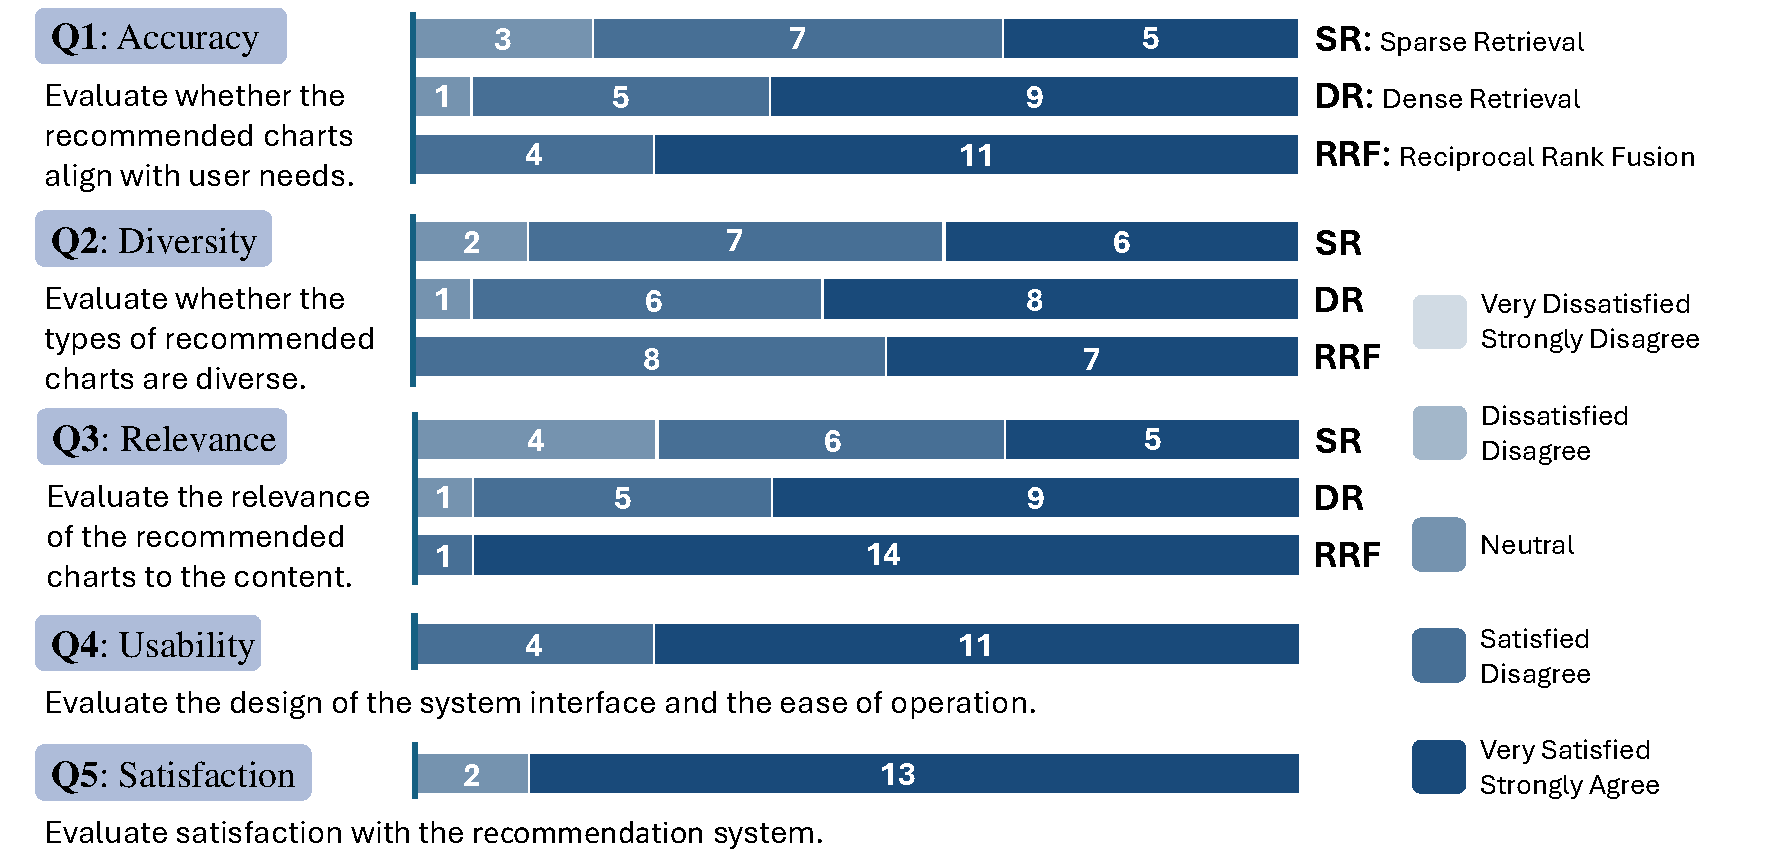
\includegraphics[width=0.8\linewidth]{pics/user_study.pdf}
    \caption{用户研究问卷结果}
    \label{fig:userstudy}
\end{figure}

本文还收集了参与者对推荐系统的开放性反馈，以更好了解其看法和建议。参与者普遍认为该系统使用起来非常方便。用户只需输入文本，系统即可推荐适合体现该文本中数值信息的图表（R1）；三种推荐算法的结果按列排列，也能够帮助数据科学初学者更好理解和解释推荐结果（R2）。参与者喜欢系统编辑区一开始给出初始图表（R5），因为这样不会削弱数据分析的乐趣。他们认为，制图不应完全自动化，因为自动化虽然可以节省体力劳动，但也可能限制创造力。通过算法和系统提供建议，帮助数据分析人员或图表制作者反复迭代和修改（R4），已经能够满足他们的需求和心理预期。

\newpage

%———————————————————————————————————————end——————————————————————————————————————————————————

%——————————————————————————————————————参考文献——————————————————————————————————————————————
	\clearpage
	\phantomsection
	\begingroup
	\bibliographystyle{gbt7714-2005-unsrt}
	\bibliography{ref}
	\endgroup
	\addcontentsline{toc}{section}{参考文献}
%———————————————————————————————————————end——————————————————————————————————————————————————



%——————————————————————————————————————致谢—————————————————————————————————————————————————		
	\makeAcknowledge{行文至此，忽觉时光匆匆，白驹过隙，犹记入学之景，却已离别之际。回首四年，承蒙恩师指导，得以一窥学术的大门；感恩学校提供的平台，让我有机会在校园里温暖地成长；感谢同学们的陪伴，让我在求知的路上不再孤单。

特别感谢我的导师孙国道老师，一开始能给我进组学习的机会，让我得以初窥可视化的世界，在后续的工作过程中，孙老师不仅在学术上给予了我细致入微的指导，还教给了令我受益匪浅的一件事，那就是要“折腾”，我愿意把这种“折腾”理解为在学术和生活中永远保持好奇。关于好奇，我想借用Alber Einstein的一句话：“The important thing is not to stop questioning. Curiosity has its own reason for existing. One cannot help but be in awe when he contemplates the mysteries of eternity, of life, of the marvelous structure of reality. It is enough if one tries merely to comprehend a little of this mystery every day.” 这种保持好奇的精神贯穿了我短短的本科生涯，也将在我未来的学术道路上给与指引。

最后感谢我的父母，把我从西部小城带到东部大都市，给我在发达地区接受高等教育的机会；感谢他们的理解和支持，让我能够专注于学业；感谢他们的爱与陪伴，让我在求学路上充满力量。}
%———————————————————————————————————————end——————————————————————————————————————————————————





%——————————————————————————————————————附录—————————————————————————————————————————————————
	% \makeAppendix{附录内容附录内容附录内容附录内容附录内容附录内容附录内容附录内容附录内容附录内容附录内容附录内容附录内容附录内容附录内容附录内容附录内容附录内容附录内容附录内容附录内容附录内容附录内容附录内容附录内容附录内容附录内容附录内容附录内容附录内容附录内容附录内容附录内容附录内容附录内容附录内容附录内容附录内容附录内容附录内容附录内容附录内容附录内容附录内容附录内容附录内容附录内容附录内容附录内容附录内容附录内容附录内容附录内容附录内容附录内容附录内容附录内容附录内容附录内容附录内容附录内容附录内容附录内容附录内容附录内容附录内容附录内容附录内容附录内容附录内容附录内容附录内容附录内容附录内容附录内容附录内容附录内容附录内容附录内容附录内容附录内容附录内容附录内容附录内容附录内容附录内容附录内容附录内容附录内容附录内容附录内容附录内容附录内容附录内容附录内容附录内容附录内容附录内容附录内容附录内容附录内容附录内容附录内容附录内容附录内容附录内容附录内容附录内容}
%———————————————————————————————————————end——————————————————————————————————————————————————

\end{document}

